% =====================================================================
%  Results chapter: architecture, optimiser, and paradigm through the
%  tangent kernel. UNIFIED draft.
%
%  Supersedes the split between the earlier kernel draft (message
%  passing in the JASTROW) and results_backflow.tex (message passing in
%  the BACKFLOW): both are the same relational-channel idea seen through
%  the tangent kernel, and are merged here. All numbers are on the
%  thesis ansatz at DMC-quality energies; seed counts are stated.
% =====================================================================
\graphicspath{{../results/figures/results/}{../results/figures/results/kernel/}{../results/figures/}}

\chapter{Architecture, optimiser, and paradigm through the tangent kernel}
\label{ch:kernel}

Our ansatz is a closed-shell Slater determinant dressed by two learnable objects:
a \emph{Jastrow}-type neural correlator $W_\theta$, which reshapes the amplitude, and a
coordinate \emph{backflow} $\Delta\mathbf{x}$, which reshapes the nodes. Each can be built in
one of two ways---without message passing, encoding and pooling per-particle and
pairwise features in a single feed-forward pass (as in a DeepSet), or as a copresheaf
\emph{message-passing} (CTNN) network that maintains explicit node and edge features and
transports information between them through learned maps before a quantity is read out
(the correlator iterates this exchange over a V-cycle; the backflow applies a single
round). The
previous chapter showed that the message-passing ansatz reaches diffusion Monte
Carlo (DMC) quality wherever a DMC reference exists ($\omega\ge0.1$), and matches
our own variational gold standard in the strongly correlated regime below it, where
no DMC benchmark is available. That settles \emph{whether} the ansatz works and
leaves the question worth a chapter: \emph{why} message passing helps at all. We
answer it for both learnable objects through a single lens, and then turn the same
lens on the optimiser and on the training paradigm.

\paragraph{One idea, one lens.} The thesis of this chapter is that message passing
buys one thing---a \textbf{relational channel}, a way to condition each particle's
contribution on where the others are---and that this single mechanism explains
three superficially separate design choices. We read all three through the geometry
of the per-sample log-derivative (score) matrix
\begin{equation}
  O_{ki} \;=\; \frac{\partial \log|\Psi_{\btheta}(\bx_k)|}{\partial \theta_i},
  \qquad k=1,\dots,B,\;\; i=1,\dots,P,
  \label{eq:kernel-O}
\end{equation}
whose Gram matrices are the quantum geometric tensor (QGT / Fisher metric)
$S = O^{\!\top}O / B$ and the neural tangent kernel $K = OO^{\!\top}$. The central
diagnostic is the \emph{effective dimension} of the variational tangent space, the
participation ratio of the QGT spectrum $\{\lambda_a\}$,
\begin{equation}
  d_{\mathrm{eff}}(S) \;=\; \frac{\left(\sum_a \lambda_a\right)^2}{\sum_a \lambda_a^2},
  \label{eq:deff}
\end{equation}
which counts how many independent tangent directions carry Fisher weight at the
solution, regardless of the parameter count $P$. We read it alongside the
local-energy variance $\Var(E_L)$ (zero only for an exact eigenstate, hence a
measure of wavefunction quality), the sampling efficiency (effective sample size
ESS), and the condition number $\kappa(S)$.

\paragraph{The three questions.}
\textbf{Q1 (architecture).} What does a message-passing correlator/backflow learn
that a separable one cannot? \textbf{Q2 (optimiser).} What does stochastic
reconfiguration (SR, natural gradient) do to the update, and where does it beat
Adam? \textbf{Q3 (paradigm).} What changes between $|\Psi|^2$-sampled VMC and
importance-sampled collocation?

\paragraph{Discipline.} Cross-architecture $d_{\mathrm{eff}}$ comparisons use a
\emph{common probe set} (all models scored on the same configurations, not on each
model's own $|\Psi|^2$); we report only participation ratios converged in the
sample count $B$; and we anchor the tooling on the analytic two-electron ground
state, where the ansatz reproduces $E=3.000127$~Ha ($+0.004\%$) with squared
overlap $1.000000$. Backflow comparisons are seeded ($\ge 2$ seeds) and held at
reference quality. Every relative error in this chapter depends on that reference,
and an external DMC benchmark exists only for $\omega\ge0.1$. In the strongly correlated regime
below, we quote errors against our own converged variational energies (the
$|\Psi|^2$-sampled SR result), and, in the deep-Wigner cascade of
\S\ref{sec:kernel-q3-frontier}, cross-check against our own fitted Wigner scaling curve
rather than any ground truth---a consistency test, since that curve is anchored on the same
unbenchmarked energies. Relative errors below $\omega=0.1$ are therefore
measures of internal consistency, not of absolute accuracy, and we read them as
such.

\paragraph{Headline findings.}
\textbf{(Q1a, Jastrow)} A message-passing correlator compresses the ground state
into $\sim\!2\times$ fewer effective tangent directions than a separable DeepSet at
weak coupling ($1.40\pm0.17$ vs $3.25\pm0.03$ at $\omega=1$, $\sim\!11\sigma$,
seeded), and those directions are the physical collective modes of $H$ (breathing,
correlation-hole, relative excitation)---to $R^2=1.00$ at the exact $N=2$ anchor, and
$R^2\!\gtrsim\!0.93$ at $N=6$ rising to $\approx\!1.00$ at $N=12$ across the confinement
range. A separable network of matched or larger capacity instead leaves nearly half its
tangent budget along directions a compact physical dictionary does not resolve---already
measurable at strong confinement, where the two networks are identical in energy.
\textbf{(Q1b, backflow)} At the Wigner crystal the \emph{conventional} backflow degrades
to $+0.5\%$ while the message-passing backflow stays at $\sim\!0.02\%$, and the structural
signature is a rank collapse: the conventional displacement field falls to a single
collective mode ($10\!\to\!1$ at $N=6$, $22\!\to\!1$ at $N=12$) where the copresheaf field
stays near its $2N$ ceiling. The reading is sharper than ``message passing helps''. Deleting
the copresheaf backflow at the crystal costs only $0.017\%$, so what message passing buys
in the nodes there is not a contribution but the \emph{absence of a pathology}: a backflow
collapsed onto one mode does not merely fail to help, it drags the nodes with it.
Q1a and Q1b are not independent: holding the
backflow fixed and varying only the correlator, its loss of physical alignment and the
backflow's rank collapse set in at the \emph{same} confinement, pointing to a common relational
bottleneck seen in the amplitude and in the nodes. \textbf{(Q2)} SR whitens the tangent
kernel; its value tracks $\kappa(S)$---negligible for the well-conditioned VMC
metric, decisive for the ill-conditioned collocation objective.
\textbf{(Q3)} VMC and collocation reach the \emph{same state} when the importance
sampling is healthy ($N=2$: overlap $>0.997$) and \emph{diverge} when it is not
($N=6$ Wigner: ESS $\to 0.11\%$ of the batch, overlap $\to 0$ under Adam). A cross-cutting caveat,
itself a result: component-level quantities (rank, $|\Delta\mathbf{x}|$) are
gauge-like. The invariants are energy, local-energy variance, and ablation---with state
overlap carrying Q3, where the two paradigms must be compared as states and not merely as
energies.

% =====================================================================
\section{Q1 --- Architecture: message passing supplies a relational channel}
\label{sec:kernel-q1}

Message passing helps in both learnable objects, in two complementary ways that are
the same statement about the tangent kernel: in the Jastrow it \emph{compresses}
the correlation into fewer effective directions; in the backflow it keeps the
displacement from \emph{collapsing} to a single direction. We take them in turn.

\subsection{Q1a --- In the Jastrow: message passing compresses the correlator}
\label{sec:kernel-q1a}

At $N=6$, $\omega=1$ the two Jastrow families are \emph{energetically
indistinguishable}: trained to DMC quality across a $20$k--$164$k parameter ladder,
every model lands within $\pm0.1\%$ of the reference, and the best raw energy
belongs to a $164$k DeepSet---twice the CTNN parameter count. Total energy is a
blunt discriminator; both have saturated the variational floor.

The difference is geometric. On a common probe set the CTNN reaches the ground
state in $d_{\mathrm{eff}}\approx1.2$--$1.7$ (three seeds), while every DeepSet
needs $d_{\mathrm{eff}}\approx2.9$--$3.6$---a factor of $\sim\!2$. The gap is robust
to the probe measure ($\lesssim0.2$ whether scored on CTNN, DeepSet, or pooled
points) and does not shrink as the DeepSet is given more capacity: the largest DeepSet in
the ladder sits at $2.9$, no lower than the smallest. The compression is
architectural, not a matter of size or sampling mass. It is also a well-posed comparison
despite $d_{\mathrm{eff}}$ not being a reparameterization-invariant absolute dimension
(\S\ref{sec:theory-tangent-kernel}): both families are compared under matched
normalisation conventions and a common probe measure, so the factor-of-two gap reflects
how each architecture spends its tangent directions, not a change of coordinates.

\begin{figure}[htbp]\centering
  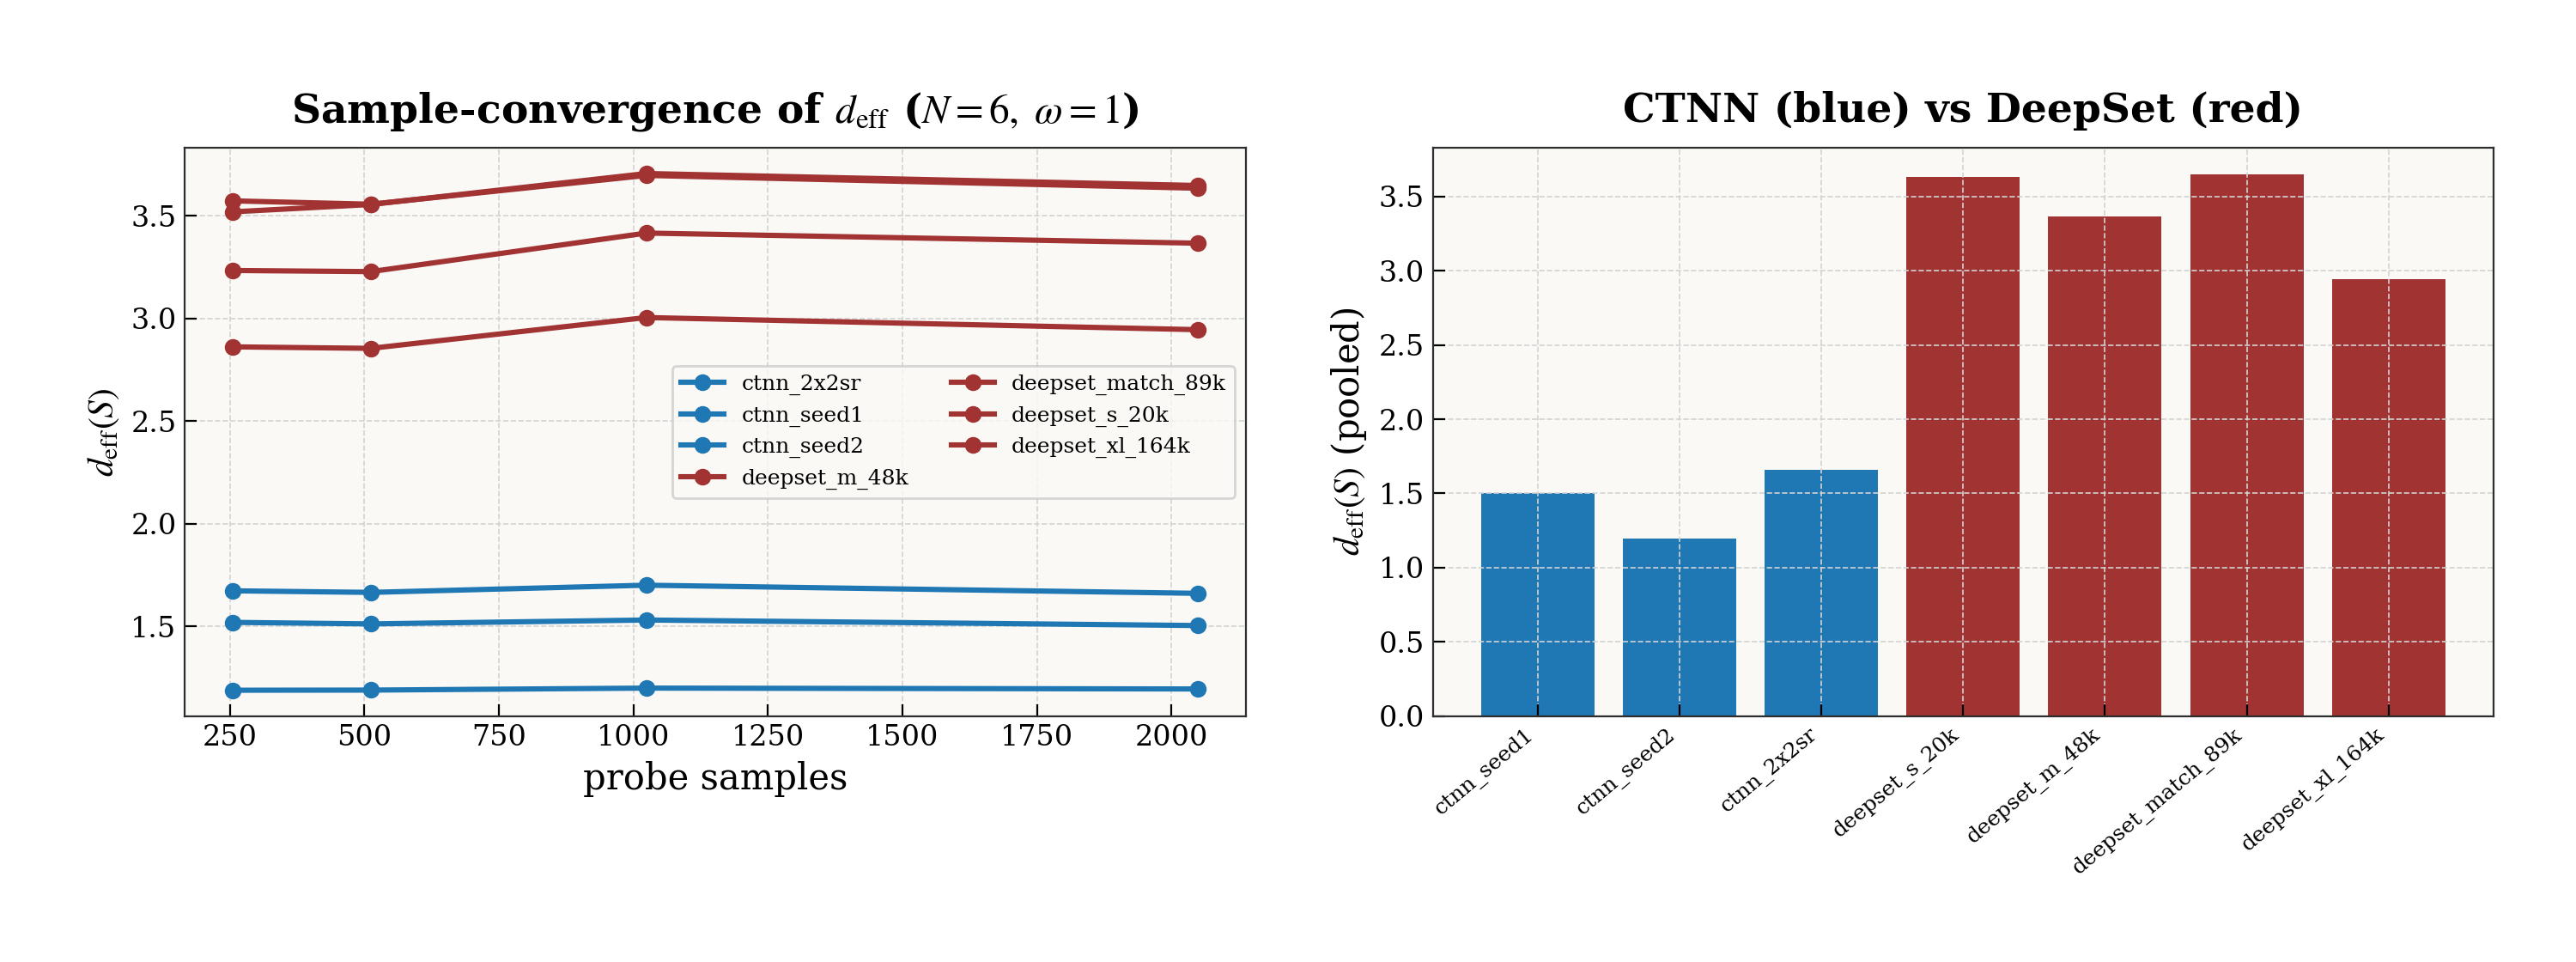
\includegraphics[width=0.95\textwidth]{fair_dimension.png}
  \caption{Message passing compresses the correlator (Q1a, $N{=}6$, $\omega{=}1$).
  \emph{Left:} the effective rank of the quantum geometric tensor on a common pooled probe,
  converged in the number of probe samples. \emph{Right:} the same pooled measure per model.
  The CTNN (blue) reaches the ground state in $d_{\mathrm{eff}}\!\approx\!1.2$--$1.7$, while
  every DeepSet (red) needs $\approx\!2.9$--$3.6$---and the gap does not close as the DeepSet
  is scaled from $20$k to $164$k parameters. The compression is architectural, not a matter
  of capacity.}
  \label{fig:q1a-fairdim}
\end{figure}

One subtlety should be dispatched here, because the synthesis
(\S\ref{sec:synthesis}) will caution that quantities split between the Jastrow and
the backflow are gauge-like. That caution does not reach this comparison: it is
between Jastrow families with \emph{no backflow present}, so there is no correlation
to divide between two substitutable channels. What remains is a comparison of how two
architectures spend their tangent directions on the same ground state, and it is
stable across seeds and across the probe measure---a property of the correlator, not
an accounting artefact.

Across seeds at fixed capacity the separation is $d_{\mathrm{eff}}=1.40\pm0.17$ (CTNN) vs
$3.25\pm0.03$ (DeepSet) at $\omega=1$, $\sim\!11\sigma$; the wider $2.9$--$3.6$ quoted
above is the spread across the \emph{capacity ladder}, not across seeds. The gap is a
\emph{strong-confinement} effect: it closes toward the Wigner crystal, where both families
reach $\sim\!3.7$ but occupy \emph{different} tangent subspaces. A single-seed dimension
``inversion'' at the crystal, reported in an earlier draft, did \emph{not} survive seeding
and is retracted here as a worked cautionary result (see \S\ref{sec:synthesis}).

\paragraph{The discriminator that survives where dimension does not.} $d_{\mathrm{eff}}$
stops separating the families at the crystal, and rank will turn out to be gauge-like
(\S\ref{sec:synthesis}). The local-energy variance does neither: it is defined on the
state, vanishes only for an exact eigenstate, and is directly comparable between any two
ansätze evaluated on their own $|\Psi|^2$. Measured at matched training protocol and
production capacity, $\Var(E_L)$ is lower for the message-passing correlator at every
confinement (Table~\ref{tab:varEL}), by factors of $2$ to $7$, while the two are
indistinguishable in energy. At the crystal the separation is clean across seeds: three
CTNN runs give $(1.95,\,1.63,\,1.96)\times10^{-5}$ against three DeepSet runs at
$(3.40,\,3.23,\,3.41)\times10^{-5}$, with no overlap. Intermediate confinements
($\omega=0.28,\,0.05,\,0.03$) reproduce the same ordering at ratios $1.2$--$1.8$. The one
place the ordering is not resolved is the smallest capacity tier used for the depth
analysis ($12$k CTNN vs $9$k DeepSet), where the two sit within $8\%$ of each other at
$\omega=1$ and $0.5$---so this is a statement about trained production models, not about
the architectures at any size.

\begin{table}[htbp]\centering
\caption{Local-energy variance at $N{=}6$, matched training protocol and production
capacity ($79.8$k CTNN vs $47.7$k DeepSet), both at reference-quality energy
($|{\rm err}|\le0.13\%$). Lower is better; $\Var(E_L)\to0$ only for an exact eigenstate.}
\label{tab:varEL}
\begin{tabular}{lccc}
\hline
$\omega$ & CTNN & DeepSet & ratio \\
\hline
$1.0$  & $1.09\times10^{-2}$ & $2.51\times10^{-2}$ & $2.3$ \\
$0.5$  & $4.62\times10^{-3}$ & $1.01\times10^{-2}$ & $2.2$ \\
$0.1$  & $5.63\times10^{-4}$ & $1.14\times10^{-3}$ & $2.0$ \\
$0.01$ & $4.11\times10^{-6}$ & $3.04\times10^{-5}$ & $7.4$ \\
\hline
\end{tabular}
\end{table}

\paragraph{Naming the manifold, at every size.} The leading tangent directions are not
abstract. At the exact $N=2$ anchor an operator decomposition identifies them, to
$R^2=1.00$, as the physical collective modes of $H$---a breathing mode
($\partial_\omega$), a correlation-hole mode, and the first relative excitation. This is not
special to two bodies. Projecting the leading tangent mode of trained correlators onto a
dictionary of physical operators (breathing/monopole, quadrupole, correlation-hole,
pair-linear), seed-averaged over well-trained checkpoints (energy within $1.5\%$ of
reference), the CTNN reaches $R^2\!\gtrsim\!0.93$ at $N=6$ and $R^2\!\approx\!1.00$ at $N=12$
across the whole confinement range $\omega\in[0.01,1]$, and both architectures reproduce the
$N=2$ naming at strong confinement (Fig.~\ref{fig:mode-naming}). The message-passing
correlator finds the ground state by moving along the handful of coordinates the Hamiltonian
actually couples.

\begin{figure}[htbp]\centering
  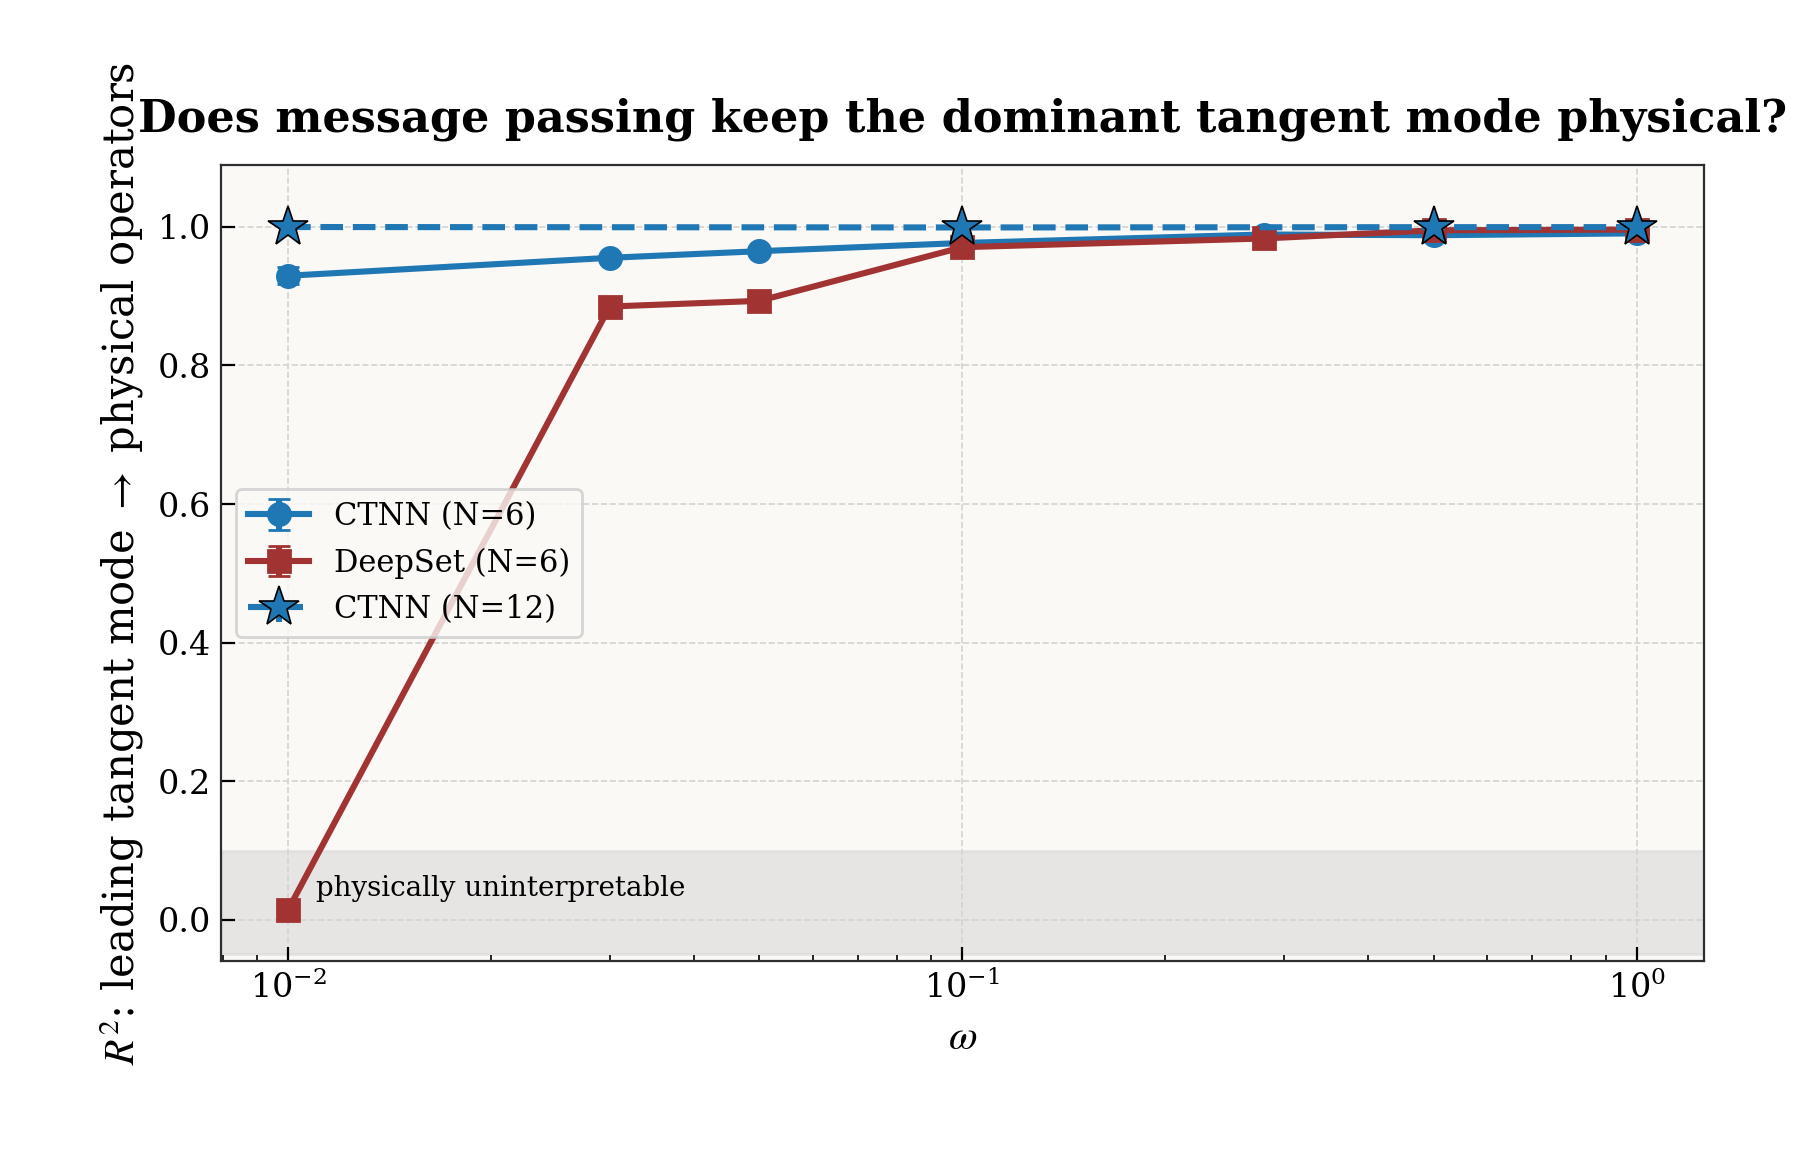
\includegraphics[width=0.8\textwidth]{mode_naming_scan.png}
  \caption{The leading tangent mode is a nameable physical mode. $R^2$ of the correlator's
  leading tangent-kernel eigenmode onto the physical-operator dictionary, seed-averaged over
  well-trained checkpoints. The CTNN stays physical at every $\omega$ and both sizes; the
  DeepSet matches it down to $\omega\!\approx\!0.1$ and then loses the leading mode entirely
  in the deep-Wigner regime. Three seeds at $\omega=0.01$.}
  \label{fig:mode-naming}
\end{figure}

\paragraph{The missing correlation channel is visible at \emph{high} $\omega$ too.} The
leading-mode score is generous to the DeepSet: at $\omega=1$ it is nominally the more physical
of the two ($R^2\!\approx\!0.996$ vs.\ $0.991$), with energies identical to four figures. Yet
a correlation-specific probe exposes a deficit the leading mode hides. Write the
eigenvalue-weighted fraction of the top tangent modes lying \emph{outside} the
physical-operator span as the \emph{dictionary-orthogonal tangent mass}. The DeepSet carries a large
excess at \emph{every} confinement---$0.44$ against the CTNN's $0.06$ at $\omega=1$, a gap of
$\sim\!0.3$--$0.5$ that persists from the strongly-confined limit down to the crystal
(Fig.~\ref{fig:nonphys}). The reading is that a separable network reaches the same energy---correlation being a small
fraction of the total at strong confinement, so the energy looks converged---while leaving
nearly half its tangent budget along directions a compact physical dictionary does not resolve.
A direction outside the dictionary need not be unphysical; the robust statement is that the
CTNN's tangent space is far more completely accounted for by a small set of physical operators
than the DeepSet's. The deficiency is intrinsic and present
throughout; weak confinement merely removes the disguise, because there correlation \emph{is}
the energy. At $N=12$ the contrast is starker still: the CTNN's dictionary-orthogonal mass stays
$\lesssim\!0.02$ across $\omega$, while a matched DeepSet (trained to $+0.2\%$) sits at
$\approx\!0.77$ at $\omega=1$---the gap \emph{widens} with system size rather than closing.

\begin{figure}[htbp]\centering
  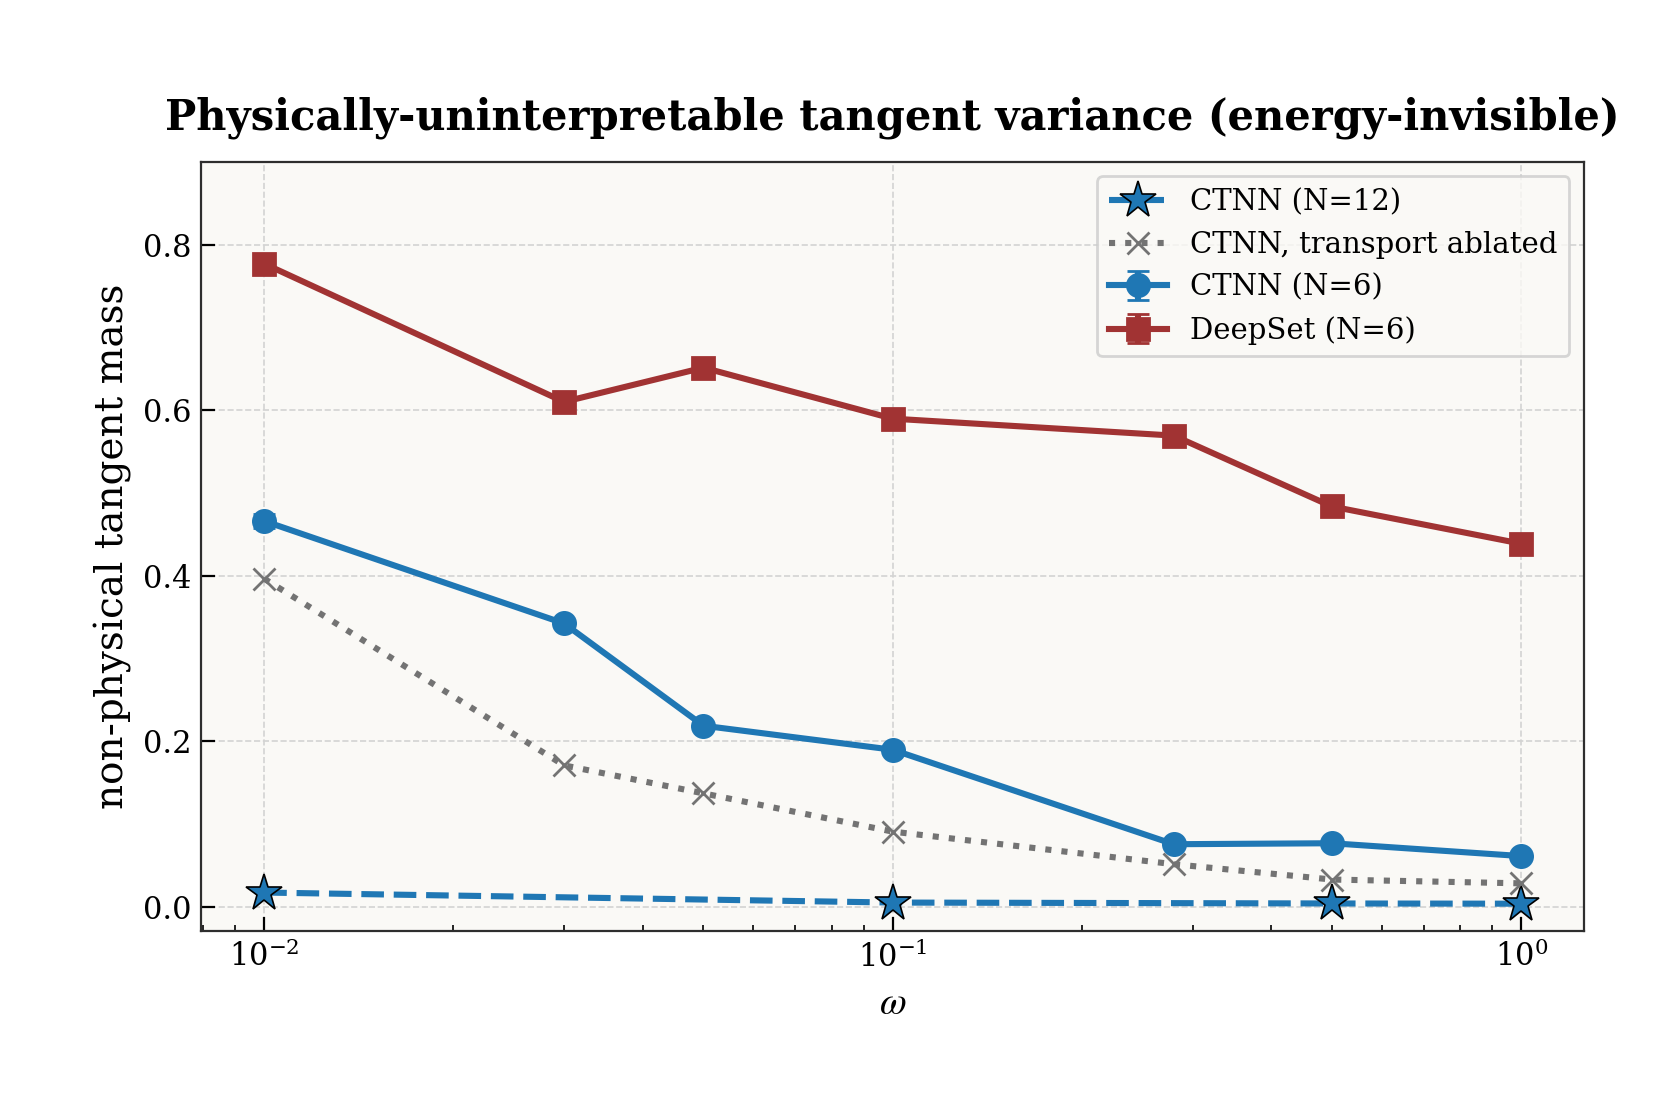
\includegraphics[width=0.72\textwidth]{nonphys_mass.png}
  \caption{A limitation visible where the energy cannot see it. Dictionary-orthogonal tangent mass---the
  eigenvalue-weighted tangent variance outside the span of a compact physical-operator
  dictionary---versus $\omega$. At
  $\omega=1$ the two correlators are indistinguishable in energy ($-0.001\%$) and in
  leading-mode physicality, yet the DeepSet already spends $44\%$ of its tangent variance on
  directions not resolved by the chosen physical-operator dictionary, against the CTNN's $6\%$. The excess is roughly constant
  in $\omega$: the correlation deficit is intrinsic, disguised at high $\omega$ only because
  correlation is a small slice of the energy there.}
  \label{fig:nonphys}
\end{figure}

\subsection{Q1b --- In the backflow: message passing prevents rank collapse}
\label{sec:kernel-q1b}

The same relational channel is decisive, in a sharper form, in the backflow. Here we
fix everything but the backflow architecture (conventional single-round messages vs.\ the copresheaf CTNN)
and train both to a Woodbury-SR endpoint. At $\omega=1$ both reach reference
quality, but they diverge as the trap weakens (Table~\ref{tab:bf_energies}): the
CTNN backflow holds $\sim\!0.02\%$ error across all $N,\omega$, while the
conventional backflow degrades to $+0.5\%$ at $N=6,\omega=0.01$ and $\sim\!6\times$
the CTNN error at $N=20,\omega=0.01$ ($+0.69\%$ vs.\ $+0.12\%$).

\begin{table}[htbp]\centering
\caption{Q1b. Relative energy error (\%), seed-averaged.}
\label{tab:bf_energies}
\begin{tabular}{l|cc|cc|cc}
\hline
 & \multicolumn{2}{c|}{$N=6$} & \multicolumn{2}{c|}{$N=12$} & \multicolumn{2}{c}{$N=20$}\\
$\omega$ & CTNN & conv & CTNN & conv & CTNN & conv \\
\hline
1.0  & $-0.03$ & $+0.06$ & $-0.01$ & $+0.04$ & $+0.06$ & $+0.07$ \\
0.1  & $-0.05$ & $+0.16$ & $+0.01$ & $+0.16$ & $+0.02$ & $+0.18$ \\
0.01 & $-0.04$ & $+0.58$ & $-0.01$ & $+0.54$ & $+0.12$ & $+0.69$ \\
\hline
\end{tabular}
\end{table}

The energy gap has a sharp structural signature. Let the \emph{backflow rank} be the
participation ratio of the displacement field $\Delta\mathbf{x}$ (how many independent
directions the backflow moves electrons along). The field lives in $2N$ dimensions, and we
project out its centre of mass (Eq.~\ref{eq:bf-com}), so the attainable ceiling is
$2N\!-\!2$: $10$, $22$, $38$ at $N=6,12,20$. Both architectures sit close to that ceiling at
large $\omega$. Toward Wigner the \emph{conventional} backflow collapses to a single
collective mode (rank $\to1$) while the CTNN backflow stays near the ceiling
(Table~\ref{tab:bf_rank}); the collapse sharpens with size ($10\!\to\!1$ at $N=6$,
$22\!\to\!1$ at $N=12$, $35\!\to\!1$ at $N=20$). The tangent dimension tells the same story
from the other side: toward Wigner $d_{\mathrm{eff}}$ grows for CTNN ($\sim\!4\!\to\!10$)
and collapses for the conventional backflow ($\sim\!6\!\to\!1$). The collapse to
\emph{exactly} rank~1 is seed-robust at every size. Rank is not the discriminator above the
crystal: at $\omega\ge0.1$ the conventional field is if anything the marginally
higher-rank of the two (Table~\ref{tab:bf_rank}), and the two architectures are then also
within $0.2\%$ of each other in energy. It is the collapse, not the level, that carries the
finding.

\begin{table}[htbp]\centering
\caption{Q1b. Backflow displacement rank (participation ratio), seed-averaged.}
\label{tab:bf_rank}
\begin{tabular}{l|cc|cc|cc}
\hline
 & \multicolumn{2}{c|}{$N=6$} & \multicolumn{2}{c|}{$N=12$} & \multicolumn{2}{c}{$N=20$}\\
$\omega$ & CTNN & conv & CTNN & conv & CTNN & conv \\
\hline
1.0  & $8.8$ & $10.4$ & $20.8$ & $22.2$ & $36.9$ & $35.4$ \\
0.1  & $7.7$ & $10.4$ & $18.2$ & $21.7$ & $33.8$ & $37.6$ \\
0.01 & $9.8$ & $\mathbf{1.0}$ & $20.8$ & $\mathbf{1.0}$ & $35.2$ & $\mathbf{1.0}$ \\
\hline
\end{tabular}
\end{table}

\paragraph{Why, mechanistically.} We price each component by ablation on a \emph{common
probe}: configurations are drawn once from the full model's $|\Psi|^2$ and every arm is
re-evaluated on them, so the trap and Coulomb terms are held fixed by construction and each
figure below is the change in the kinetic term at fixed measure---the instantaneous cost of
removing a component, not the energy of a re-relaxed state. Two facts are seed-stable.
(i) The \textbf{relational work migrates from the nodes to the amplitude} as the trap
weakens. Deleting the backflow costs $+5.6\%$ at $\omega=1$ and $+1.4\%$ at $\omega=0.1$,
but only $+0.013$--$0.017\%$ at $\omega=0.01$ (three seeds), while deleting the Jastrow
messages runs the other way: $+3.9\%$ at $\omega=1$ rising to $+9$--$15\%$ at
$\omega=0.01$. At the crystal the backflow is very nearly inert---with the Jastrow messages
already removed, deleting the displacement as well changes the energy by under $0.01\%$.
``Message passing buys kinetic energy through the nodes'' is a high-$\omega$ statement only.
(ii) \textbf{Within the backflow, the transport maps \emph{are} the displacement}: zeroing
the inter-particle transport maps ($\rho_{v\to e},\rho_{e\to v}$) perturbs
$\Delta\mathbf{x}$ by as much as deleting it outright---the mean
$|\Delta\mathbf{x}_{\mathrm{abl}}-\Delta\mathbf{x}|$ is comparable to the mean
$|\Delta\mathbf{x}|$ at every $(N,\omega)$---so what displacement the network produces comes
from the messages rather than from the per-particle path. Both architectures condition each particle on the
relative coordinates $\mathbf r_{ij}$, so neither is blind to inter-particle structure;
the difference is that the conventional backflow uses a single round of pairwise
messages aggregated per particle, whereas the CTNN maintains and transports explicit
edge state across the graph. Empirically the single-round backflow does not
\emph{sustain} a full-rank relative displacement at the crystal---it collapses to a
single collective displacement mode (rank~1)---while the CTNN's copresheaf transport holds the full-rank
response, and the ablation shows that this transport carries essentially the entire
effect.

\begin{figure}[htbp]\centering
  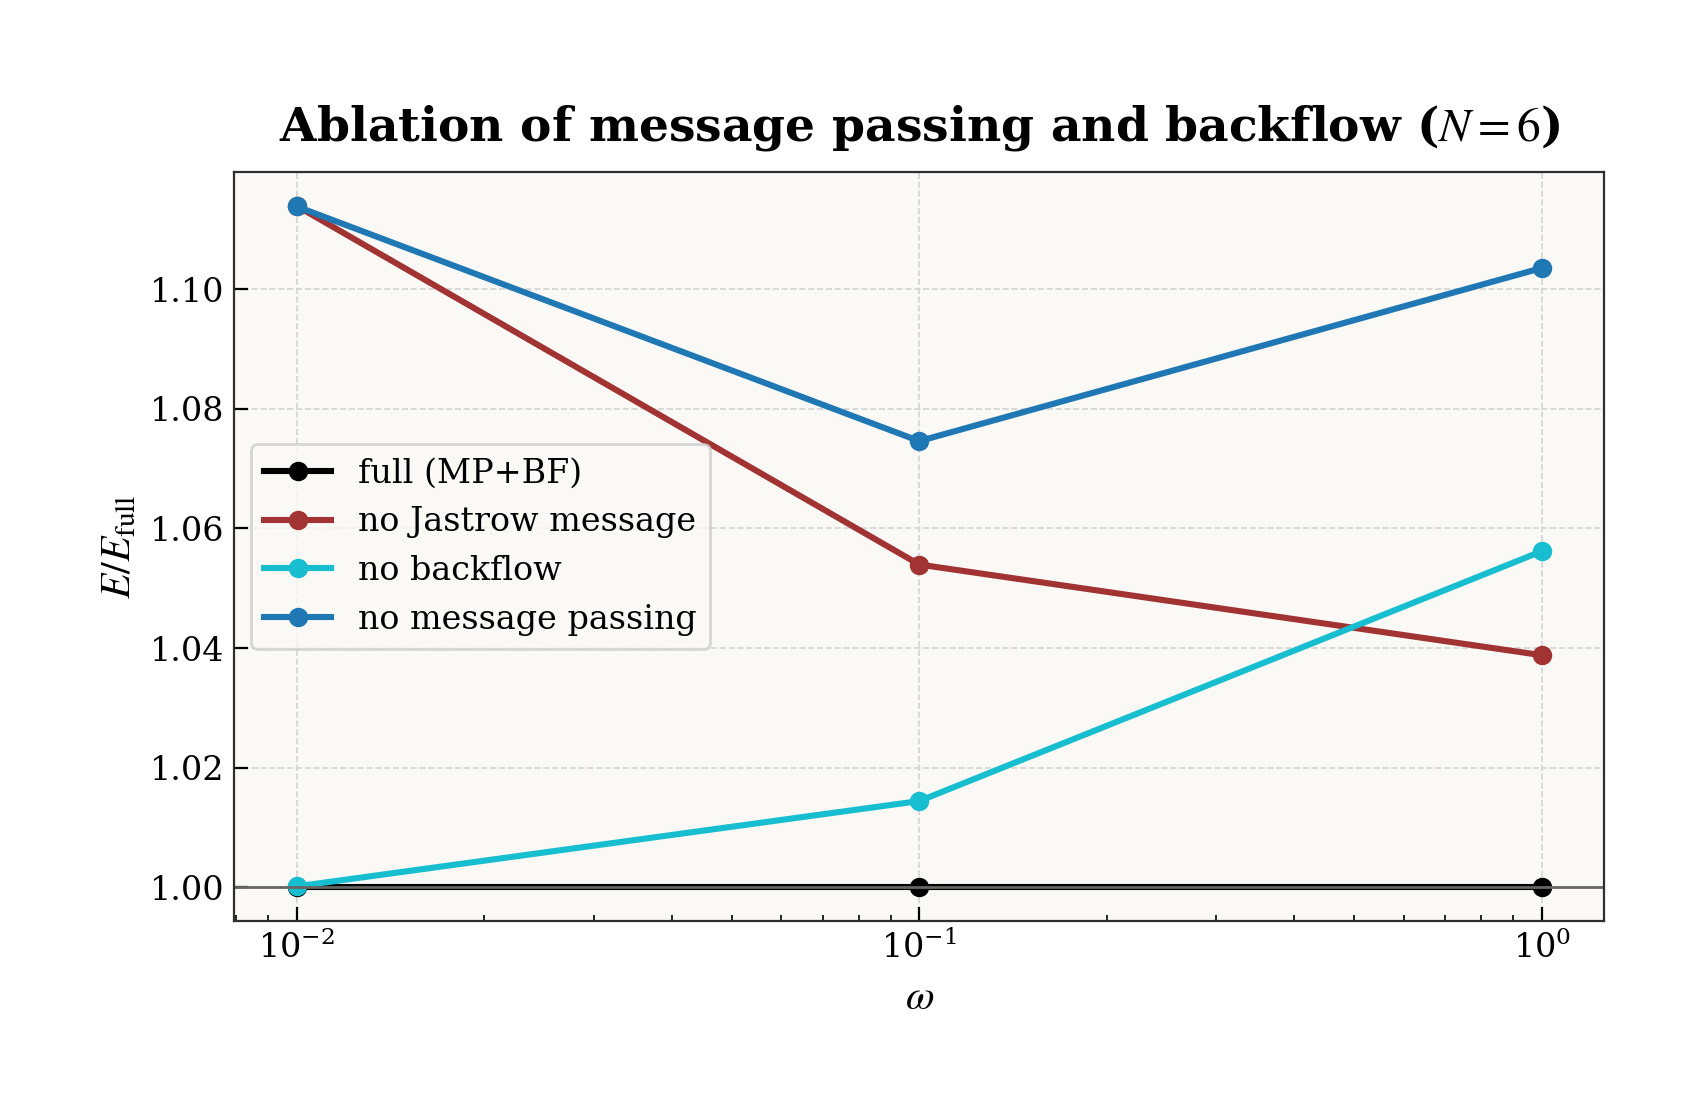
\includegraphics[width=0.72\textwidth]{message_ablation.png}
  \caption{What message passing buys, by ablation (trained networks, $N{=}6$; energy
  relative to the full model, all arms evaluated on a common probe drawn from the full
  model's $|\Psi|^2$). Removing the backflow (orange) costs $\sim\!6\%$ at $\omega{=}1$ but
  under $0.02\%$ at $\omega{=}0.01$, while removing the Jastrow messages (red) or all
  message passing (blue) grows more expensive as the trap weakens. The relational work
  migrates from the nodes to the amplitude: at the crystal it is the correlator's messages,
  not the backflow, that carry it.}
  \label{fig:q1b-ablation}
\end{figure}

\subsection{The unified reading of Q1}
Q1a and Q1b are one statement about how relational information is \emph{routed}. The
baselines are not blind to inter-particle structure---the DeepSet pools
independently-encoded pairs, and the conventional backflow aggregates a single round of
pairwise messages---but neither maintains a persistent, transported edge representation:
each pairwise term is computed and discarded. The copresheaf CTNN does maintain one, and
moves it back and forth between nodes and edges through learned transport maps
($\rho_{v\to e},\rho_{e\to v}$); the message-passing correlator iterates this exchange over
a V-cycle, while the backflow applies a single such copresheaf round. Where a compact
representation exists this \emph{compresses} the correlation onto fewer tangent directions
(Jastrow: smaller $d_{\mathrm{eff}}$); where the physics demands a genuinely collective,
full-rank response the single-round baseline instead collapses to a single collective
displacement mode (backflow: rank~1), which the copresheaf transport avoids. Both effects are visible only
in the tangent-kernel geometry, not in the total energy, until weak confinement makes
the geometric deficit an energetic one.

\paragraph{The two channels fail together.} The correlator deficit and the backflow
deficit set in at the \emph{same} confinement. Holding
the backflow architecture fixed (the conventional network, in both cases) and varying only the
correlator, we track the correlator's correlation-hole capture and the backflow's displacement
rank down the $\omega$-sweep (Fig.~\ref{fig:q1-unify}). With a DeepSet correlator both give way
together at $\omega\!\approx\!0.05$---the hole capture falls from $0.68$ to $0.07$ as the
backflow rank drops from $\sim\!10$ to $1$. With a CTNN correlator both hold until
$\omega\!\approx\!0.01$. The correlator's grip on the physical correlation modes and the
backflow's ability to sustain a full-rank displacement are the same capability seen from two
sides: when the amplitude model can no longer resolve the correlation hole, the nodal
deformation can no longer stay high-rank, and a better correlator postpones \emph{both}. The
evidence---coincident transitions that shift together under a correlator swap---supports a
common relational bottleneck underlying Q1a and Q1b rather than proving them literally identical.

\begin{figure}[htbp]\centering
  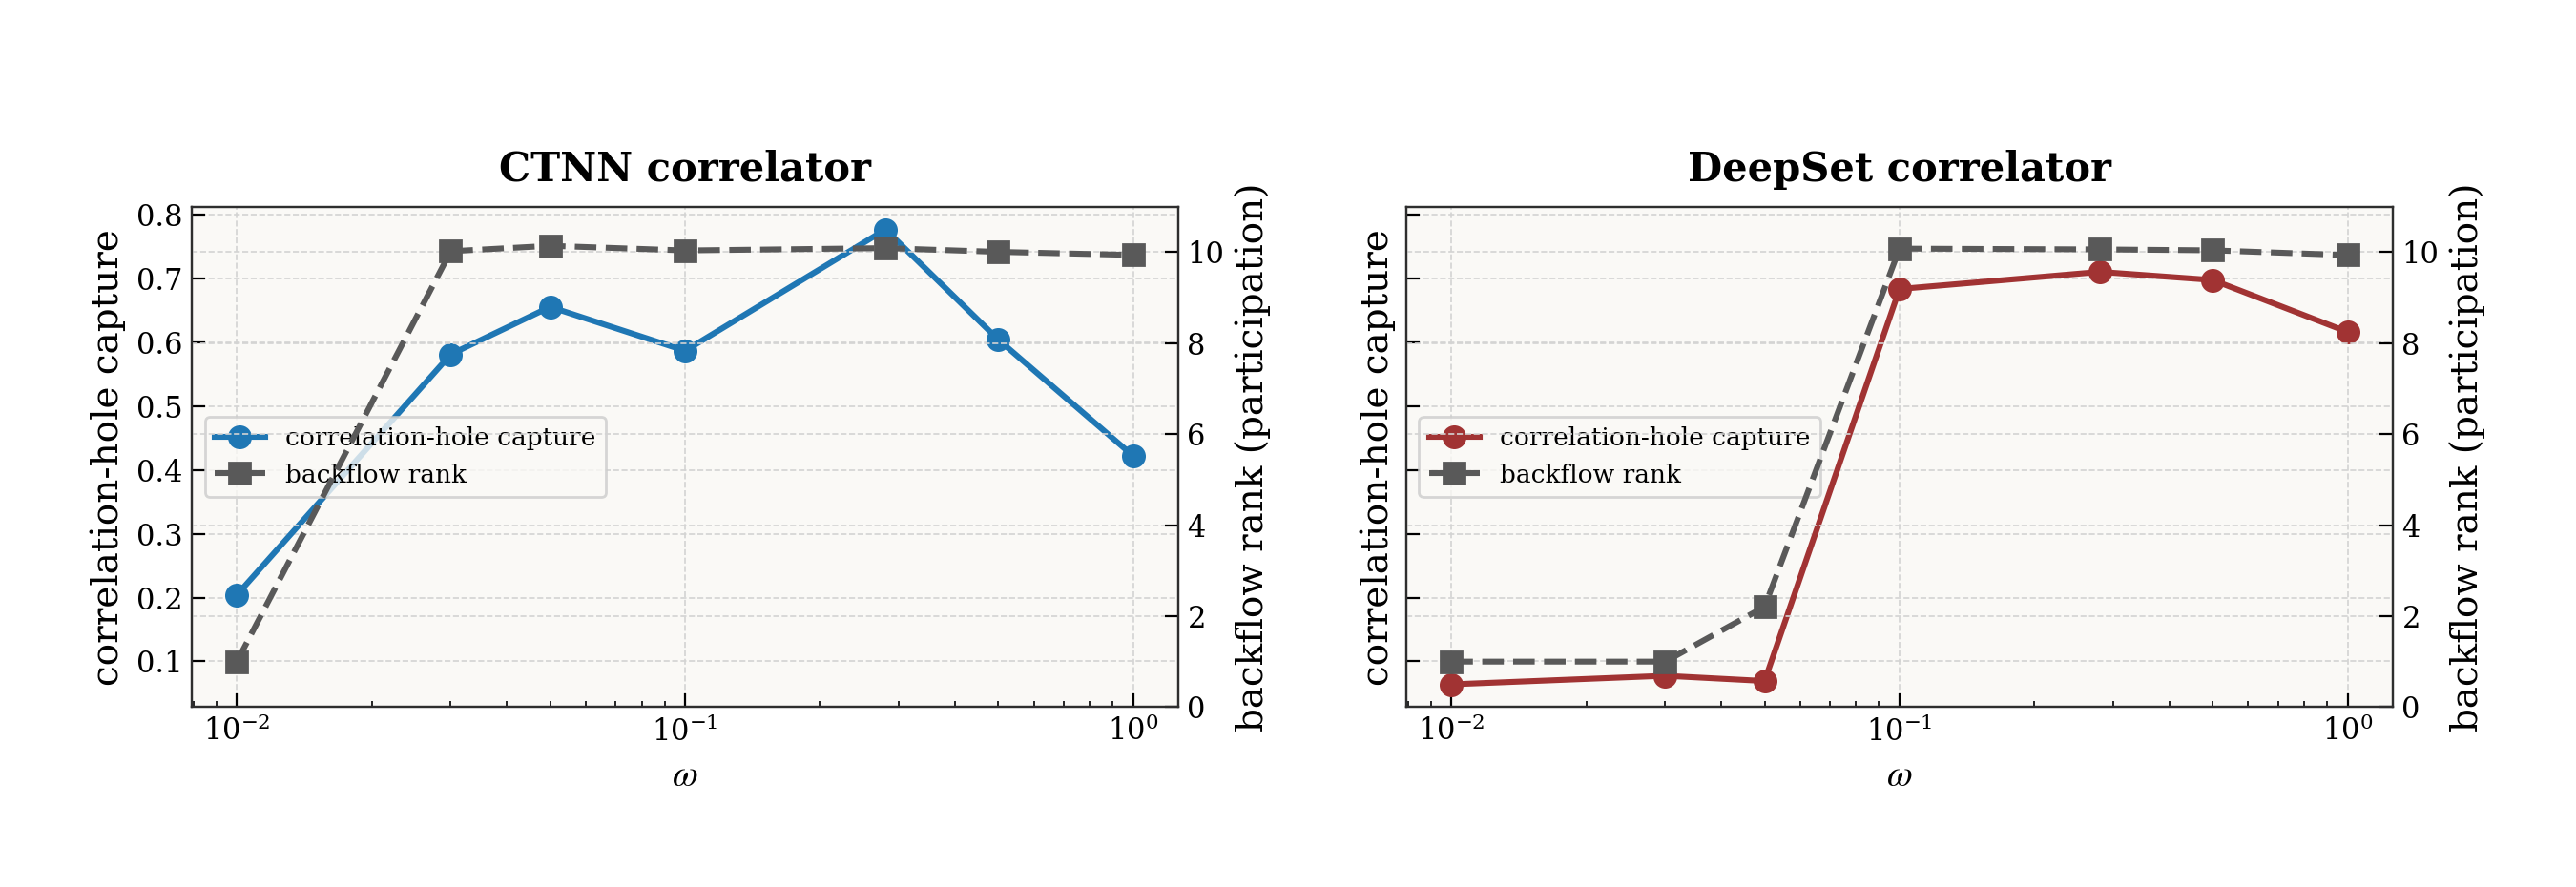
\includegraphics[width=\textwidth]{q1_unification.png}
  \caption{Correlator physicality and backflow rank collapse together ($N=6$; the backflow
  architecture is held fixed, only the correlator changes). For each correlator, the
  correlation-hole capture (left axis) and the backflow displacement rank (right axis) give way
  at the same $\omega$: $\omega\!\approx\!0.05$ for the DeepSet, $\omega\!\approx\!0.01$ for the
  CTNN. A correlator that keeps its physical structure lets the backflow keep its rank.}
  \label{fig:q1-unify}
\end{figure}

% =====================================================================
\section{Q2 --- Optimiser: SR earns its keep where the metric is ill-conditioned}
\label{sec:kernel-q2}

Stochastic reconfiguration preconditions the gradient by the inverse QGT,
$\btheta \leftarrow \btheta - \eta\, S^{-1}\nabla_{\btheta} E$; geometrically it \emph{whitens} the tangent
kernel. At $N=2$ this is exact: the SR step aligns with the imaginary-time direction
to numerical precision. The question is where whitening changes the outcome.

Fixing the ansatz and varying only the optimiser from a common stage-3 base:
\textbf{for $|\Psi|^2$-VMC, SR and Adam are indistinguishable}---exact at $N=2$
(var $\sim\!10^{-9}$), and at $N=6$ the energy gap
$E_{\mathrm{Adam}}-E_{\mathrm{SR}}$ is $\lesssim0.002$ across $\omega$ and both
seeds. The VMC metric is well enough conditioned ($\kappa(S)$ moderate, and
$|\Psi|^2$ sampling is self-preconditioning) that Adam already moves along the right
directions. \textbf{For weak-form collocation, SR is essential}: there
$E_{\mathrm{Adam}}-E_{\mathrm{SR}}$ is large and positive (e.g.\ $+2.9$ at
$N=6,\omega=1$), because the importance weights make the objective badly
conditioned and plain Adam fails to converge it.

The verdict is therefore not ``SR wins'' or ``SR ties'' but \textbf{SR matters when
the tangent metric is ill-conditioned and still estimable}. Its value is a
function of $\kappa(S)$, set by the ansatz and the sampling measure, not an intrinsic
property of the optimiser---which is exactly why an earlier low-$\omega$ VMC sweep
saw a modest SR advantage that never grew into a decisive win.

The claim needs one sharpening, because ``more ill-conditioned $\Rightarrow$ more
useful SR'' cannot hold without bound: inverting $S$ requires $S$ itself to be
\emph{reliably estimated}. SR helps when the tangent metric is anisotropic but its
empirical estimate is trustworthy; once the sampling that builds $S$ collapses---as the
importance weights do deep in the Wigner regime---the empirical $S$ becomes noisy and
rank-deficient, and preconditioning by its inverse amplifies that noise rather than the
signal. This is exactly the behaviour seen at ultra-weak confinement, where CG-SR on the
collocation objective becomes unstable (Chapter~\ref{ch:results},
\S\ref{sec:colloc-negatives}): not a counterexample to the conditioning story but its
completion---SR pays off in the window where the metric is both ill-conditioned and
estimable, and fails once estimation itself breaks down.

One further boundary deserves to be drawn explicitly. The VMC equivalence of
Adam and SR is established here at $N=2$ and $N=6$; we have not verified that it
survives to $N=12$ and $N=20$, where the conditioning of the VMC metric could in
principle worsen with dimension. The mechanism we propose---that $|\Psi|^2$ sampling
keeps $\kappa(S)$ moderate and so lets Adam's diagonal preconditioning suffice---is a
prediction there, not yet a measurement, and testing it is the obvious extension.

% =====================================================================
\section{Q3 --- Paradigm: the sampling measure sets conditioning, variance, and reach}
\label{sec:kernel-q3}

Between $|\Psi|^2$-VMC and importance-sampled collocation the wavefunction family is
identical; only the measure that defines the loss changes. Three consequences, one
statement.

\paragraph{$|\Psi|^2$ is self-preconditioning; the covering proposal is not.}
Sampling from $|\Psi|^2$ makes the estimator of $S$ and of the gradient share the
same measure, which conditions the update. A fixed covering proposal instead drives
a monotone \emph{ESS collapse} as $N$ and $1/\omega$ grow: at $N=6,\omega=0.01$ the
effective sample size falls to $0.11\%$ of the batch (about $5$ of the $4096$ retained
points---the normalisation used for every ESS figure in this thesis). When ESS collapses the
gradient estimator is degenerate---a hard limit, not undertraining.

This needs one reconciliation, because Chapter~\ref{ch:results} reports usable collocation
energies at the same $(N,\omega)$ where the estimator is called degenerate here
($+0.24$--$0.29\%$ across three seeds, Table~\ref{tab:reliability}). Two things differ.
First, the sampler: the collapse measured above is for the \emph{static} origin-centred
mixture, while the campaign's robust recipe refits its proposal every $30$ epochs and
oversamples $16\times$. The campaign's \emph{baseline} rows, which keep the static
proposal, are the ones that blow up ($+3.9$ to $+7.2\%$ at $\omega=0.001$). Second, and
more interesting, the two statements are not about the same quantity. The energy stays
within a third of a percent while the state overlap goes to zero---which is the sharpest
illustration in this thesis of why energy alone does not certify a state. The honest
qualification is that $\mathcal{S}^2$ is itself a ratio estimator built from the same
degenerate weights, so ``$\to0$'' should be read as \emph{unresolvable at this ESS} rather
than as a measured orthogonality.

\begin{figure}[htbp]\centering
  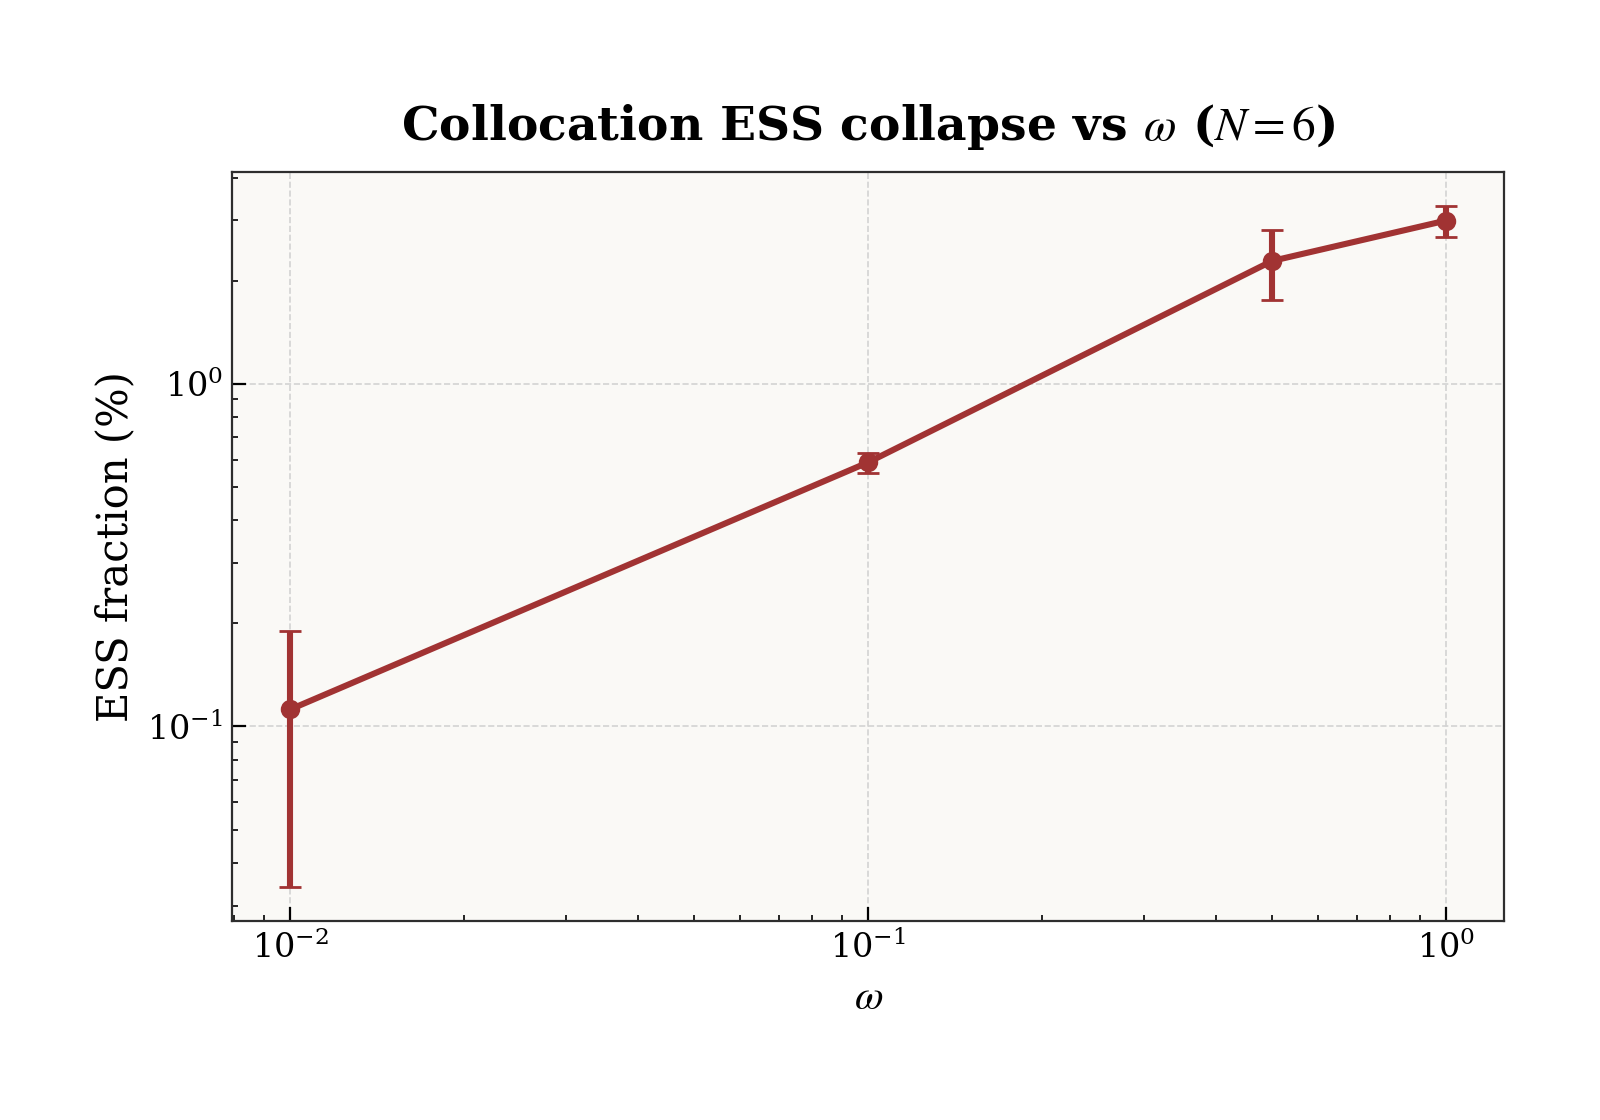
\includegraphics[width=0.62\textwidth]{ess_collapse.png}
  \caption{The naive collocation proposal collapses in the Wigner regime ($N{=}6$). The
  effective sample size (as a percentage of the batch) falls by more than an order of
  magnitude from $\omega{=}1$ to $\omega{=}0.01$, where it reaches $\sim\!0.1\%$---about five
  usable points in a batch of $4096$. This is a property of the sampling measure, not of
  optimisation, and it is what the physics-informed ring proposal
  (\S\ref{sec:kernel-q3-frontier}) is designed to repair.}
  \label{fig:q3-ess}
\end{figure}

\paragraph{Same state, until the sampling loses the target.} We test whether the two
paradigms reach the same \emph{state} (not merely the same energy) via the symmetric
overlap
$\mathcal{S}^2=\langle\Psi_B/\Psi_A\rangle_{|\Psi_A|^2}
\langle\Psi_A/\Psi_B\rangle_{|\Psi_B|^2}$. At $N=2$ they are identical
($\mathcal{S}^2>0.997$ for every $\omega$, both optimisers, both seeds): the paradigm
is efficiency-only, collocation paying $\sim\!5\times$ the variance for the same
wavefunction. At $N=6$ they \emph{diverge}: under Adam $\mathcal{S}^2$ falls
$0.85\to0.77\to\approx0$ from $\omega=1$ to $0.01$ (both seeds), tracking the ESS
collapse; SR partially rescues it ($\mathcal{S}^2\!\approx\!0.95$) but does not close
the gap. Weak-form collocation thus has a \textbf{domain of validity}---equivalent to
VMC when the importance sampling is healthy, degrading as correlation strengthens.
This couples Q3 to Q2: the paradigm that needs SR is the one that breaks down at
scale. An adaptive proposal that tracks $|\Psi|^2$ is the natural remedy, pursued in
\S\ref{sec:kernel-q3-frontier}.

\paragraph{Why the collocation energy readout is biased.} For an exact eigenstate the
local energy $E_L=\hat H\Psi/\Psi$ is constant over configuration space, so
$\Var(E_L)\to0$ as the ansatz approaches the ground state---the zero-variance principle,
and the reason $\Var(E_L)$ is a sharp quality measure. That cancellation is a property of
the \emph{full} local energy, in which the kinetic (Laplacian) and potential terms combine
to a constant; it is not a property of the Laplacian term alone. The collocation objective
does \emph{not} discard the Laplacian: it is a score-function (REINFORCE) estimator that
\emph{forms} the full $E_L$ as a detached reward and differentiates only $\log|\Psi|$
(\S\ref{sec:colloc-method}). What it gives up is the \emph{measure}: the reward is averaged
over the analytic proposal with importance weights (and, in the hardest regimes, tempered
weights), so the importance-sampled energy \emph{readout} is a biased estimate of
$\langle E_L\rangle_{|\Psi|^2}$ and must not be used as the convergence criterion. The
reliable criteria are $\Var(E_L)$ and the state overlap, both evaluated on $|\Psi|^2$
samples.

% =====================================================================
\section{The collocation frontier: a physics-informed proposal for the Wigner regime}
\label{sec:kernel-q3-frontier}

The ESS collapse of \S\ref{sec:kernel-q3} is a limitation of the \emph{proposal}, not
of collocation itself, and it can be substantially pushed back. This section reports a
physics-informed proposal that extends MCMC-free collocation deep into the Wigner
regime, the mechanism that limits it, and the wall that remains.

\subsection{The origin-centred proposal misses the Wigner shell}
Every proposal in the standard pipeline is a mixture of \emph{origin-centred} Gaussians
$q(\mathbf{R})=\frac1K\sum_k \mathcal{N}(\mathbf{R};0,\sigma_{f,k}^2/\omega)$. But as
$\omega\to0$ the electrons localise into a Wigner molecule on a \emph{shell} far from the
origin: the classical $N=6$ minimum is the $(1,5)$ configuration---one central electron,
five on a ring at radius
$1.334\,\omega^{-2/3}$~\cite{schweigert1994spectralpropertieschargedparticles,Kong_2002}---which
in oscillator units sits at
$1.96/2.87/4.22\,\ell$ for $\omega=0.1/0.01/0.001$, moving outward as the trap weakens,
past the reach of a width-$2\ell$ origin Gaussian. The proposal aims where $|\Psi|^2$ has
no mass; hence the collapse.

\subsection{The Wigner-ring proposal}
We replace the origin mixture with a \emph{Wigner-ring} proposal: a radial Gaussian at the
shell radius times an angular distribution for the ring electrons, plus a central Gaussian.
On trusted states this lifts the effective sample size by $15$--$47\times$ over the origin
mixture (Table~\ref{tab:ring-ess}), turning a collapsed sampler into a usable one---without
any training, a cheap decisive test. Fitting the ring to $|\Psi|^2$ samples (the simplest
adaptive form) doubles the ESS again; a $(1,5)+(0,6)$ mixture \emph{hurts} at $N=6$, since
the state is $(1,5)$ and the extra channel dilutes the proposal mass.

\begin{table}[htbp]\centering
\caption{ESS (of 4096) against a trusted $N=6,\omega=0.01$ state. The origin mixture is
already collapsed; the ring proposal covers the shell.}
\label{tab:ring-ess}
\begin{tabular}{lc}
\hline
proposal & ESS \\
\hline
origin-Gaussian mixture (standard) & $1.5$ \\
Wigner ring $(1,5)$, hand-tuned & $22.5$ \\
Wigner ring $(1,5)$, fitted to $|\Psi|^2$ & $47.5$ \\
\hline
\end{tabular}
\end{table}

\subsection{Angular crystallisation is the deep-Wigner wall}
Why does the ring work at $\omega=0.01$ but fail at $\omega=0.001$? The molecule
\emph{crystallises angularly} as the trap weakens. The nearest-neighbour angular-gap
standard deviation of the five ring electrons is $40.8^\circ/33.3^\circ/25.5^\circ/6.7^\circ$
at $\omega=1/0.1/0.01/0.001$: a ``ring liquid'' at moderate coupling becomes an angular
crystal (electrons pinned near $72^\circ$ apart) at $\omega=0.001$. A proposal with
independent, uniform angles almost never lands on the crystalline configuration---so the
angular distribution must crystallise too. This is captured MCMC-free by modelling the five
gaps (which sum to $2\pi$) as $\mathrm{Dirichlet}(\alpha)$: an exact tractable density whose
single concentration $\alpha$ interpolates liquid ($\alpha$ small) to crystal ($\alpha$
large), fitted to the measured gap variance. This diagnosis \emph{explains} the collocation
wall that is otherwise only observed.

\subsection{An MCMC-free cascade reaches $\omega=0.0035$}
Combining the ring proposal (radial Gaussian $\times$ Dirichlet gaps) with importance
oversampling, a \emph{continuous} adaptive re-fit of the proposal to the current
importance-weighted batch (every few steps, no MCMC), and a gentle $\omega$-cascade
seeded from a converged $\omega=0.01$ state, MCMC-free collocation produces states that
lie on the Wigner energy-scaling curve down to $\omega=0.0035$---four cascade rungs, with
heavy-VMC energies within $1$--$2\%$ of the scaling estimate (Table~\ref{tab:cascade}),
well past where the origin proposal collapses ($\mathrm{ESS}\!\approx\!1.5$ of $4096$ at
$\omega=0.01$, Table~\ref{tab:ring-ess}). The essential ingredient is the continuous re-fit: it keeps ESS healthy
($\sim\!10^2$) \emph{while} the energy descends, where a static or slowly-updated proposal
collapses to $\mathrm{ESS}\!\sim\!1$ as the wavefunction moves away from it.

\begin{table}[htbp]\centering
\caption{MCMC-free Wigner-ring cascade, $N=6$: heavy-VMC energy vs.\ the fitted Wigner
scaling curve $E(\omega)\approx 0.690\,(\omega/0.01)^{0.689}$, whose exponent is close to
the classical $2/3$ but whose prefactor is anchored at $\omega=0.01$, where no external
reference exists. The agreement is therefore internal consistency, not validation. Good to
$\omega=0.0035$.}
\label{tab:cascade}
\begin{tabular}{lccc}
\hline
$\omega$ & $E$ & scaling est. & ratio \\
\hline
0.0077 & 0.577 & 0.577 & 1.00 \\
0.0059 & 0.481 & 0.480 & 1.00 \\
0.0045 & 0.400 & 0.398 & 1.01 \\
0.0035 & 0.340 & 0.335 & 1.02 \\
\hline
\end{tabular}
\end{table}

\subsection{The remaining wall: a fine-tuned Slater--Jastrow balance, not the sampler}
Below $\omega=0.0035$ the cascade becomes unstable, and---informatively---the instability
is \emph{non-monotonic} across proposal variants: wide-exploratory, tempered-tracking, and
outward-anchored proposals each converge some rungs and diverge others. That pattern
locates the obstacle not in the proposal but in the warm-start, and four transfer diagnostics
(taking the converged $\omega=0.0035$ rung down to $\omega=0.0027$, a $23\%$ step) pin down
its mechanism precisely.

First, the frontier state is genuine: at its own $\omega=0.0035$ the rung is a bona-fide
Wigner molecule, with radial density peaked at $3.34\ell$ (classical ring $3.42\ell$) and a
\emph{single} basin---initialising the sampler on the shell converges to the same $3.34\ell$.
Transferred to $\omega=0.0027$, however, the wavefunction collapses to $\sim\!1\ell$, and two
tests show \emph{where} the collapse lives. It is not the sampler: initialising the Metropolis
walkers directly on the classical shell ($3.57\ell$) still relaxes inward to $1.1\ell$, so the
collapsed density is a property of the ansatz, not of sampler initialisation. And it is not the
backflow: its displacement is small ($|\Delta\mathbf{x}|\approx0.13\ell$, radially inward) and
essentially \emph{preserved} across the transfer ($0.15\ell\!\to\!0.13\ell$)---it scales
correctly with $\ell$ but is far too small to bridge the $2.4\ell$ gap between the Slater core
($\sim\!1\ell$) and the Wigner shell.

The mechanism is a delicate cancellation. The bare harmonic-oscillator determinant suppresses
the shell by $\exp(-\omega r^2/2)\!\sim\!\exp(-5.6)$ in amplitude ($\sim\!10^{-5}$ in density);
the Wigner peak exists only because the Jastrow amplifies it back by a comparable factor, with
the backflow contributing a small inward nudge. A $23\%$ change in $\omega$ perturbs both the
Slater confinement and the Jastrow correlation length, the fine-tuned balance tips, and the
density falls back to the non-interacting shell---from which the collocation re-fit cannot
reliably climb out (hence the non-monotonic proposal behaviour). This rules out the natural fix
of an $\omega$-robust warm-start by coordinate rescaling: because the ansatz relaxes inward even
when handed shell configurations, no coordinate transform can preserve the state. Reaching
$\omega<0.0035$ would require per-$\omega$ re-optimisation against a shell-\emph{amplitude}-anchored
objective, or a genuinely $\ell$-covariant parametrisation---a distinct problem left to future
work. The contribution here is concrete: a physics-informed proposal that carries MCMC-free
collocation from the origin-proposal wall down to a verified Wigner molecule at $\omega=0.0035$,
and a precise account of the angular-crystallisation and Slater--Jastrow-balance effects that
bound it.

% =====================================================================
\section{Synthesis and discussion}
\label{sec:synthesis}

The three axes are one geometry. Architecture sets the shape of the tangent space
(message passing compresses it in the Jastrow, and keeps it from collapsing in the backflow);
the optimiser inverts the metric on that space (SR pays off only when it is ill-conditioned);
and the paradigm chooses which measure defines the metric ($|\Psi|^2$ self-preconditions and
stays on target, while the covering proposal loses conditioning and eventually the state). The
single cross-cutting discriminator, robust where dimension and rank are not, is $\Var(E_L)$:
at matched protocol and production capacity it is lower for the message-passing ansatz at
every $\omega$ by factors of $2$--$7$ (Table~\ref{tab:varEL}), seed-cleanly so at the
crystal, and it says so where energy cannot and where $d_{\mathrm{eff}}$ has stopped
separating the families. What this geometry means for the
physics, and how the threads combine, is taken up in the Discussion (Chapter~\ref{ch:discussion})
and Conclusion.

\paragraph{A gauge caveat, itself a result.} Component-level quantities---backflow
rank, displacement magnitude $|\Delta\mathbf{x}|$, per-component
$d_{\mathrm{eff}}$---are \textbf{gauge-like}. The Jastrow and backflow are
substitutes, so how correlation is split between them is a nearly-flat,
path-dependent direction of the loss; those quantities depend on the training route,
not on the state. Every claim that reversed during this project was of that kind
(the retracted $d_{\mathrm{eff}}$ inversion at the crystal; a mislabelled backflow;
an artefactual rank collapse from joint-from-scratch training). The reliable
measurements---energy, state overlap, and ablation (delete a component, price it in
energy)---are invariant to the gauge, together with $\Var(E_L)$, and the conclusions
above rest only on those. Their division of labour is worth stating plainly: energy and
ablation carry Q1, $\Var(E_L)$ separates the architectures where energy and dimension no
longer can, and state overlap is what makes Q3 a claim about states rather than about
numbers that happen to agree.
